\documentclass[14pt]{beamer}
\usepackage{./Estilos/BeamerUVM}
\usepackage{./Estilos/ColoresLatex}
\usetheme{Madrid}
\usecolortheme{default}
%\useoutertheme{default}
\setbeamercovered{invisible}
% or whatever (possibly just delete it)
\setbeamertemplate{section in toc}[sections numbered]
\setbeamertemplate{subsection in toc}[subsections numbered]
\setbeamertemplate{subsection in toc}{\leavevmode\leftskip=3.2em\rlap{\hskip-2em\inserttocsectionnumber.\inserttocsubsectionnumber}\inserttocsubsection\par}
% \setbeamercolor{section in toc}{fg=blue}
% \setbeamercolor{subsection in toc}{fg=blue}
% \setbeamercolor{frametitle}{fg=blue}
\setbeamertemplate{caption}[numbered]

\setbeamertemplate{footline}
\beamertemplatenavigationsymbolsempty
\setbeamertemplate{headline}{}


\makeatletter
% \setbeamercolor{section in foot}{bg=gray!30, fg=black!90!orange}
% \setbeamercolor{subsection in foot}{bg=blue!30}
% \setbeamercolor{date in foot}{bg=black}
\setbeamertemplate{footline}
{
  \leavevmode%
  \hbox{%
  \begin{beamercolorbox}[wd=.333333\paperwidth,ht=2.25ex,dp=1ex,center]{section in foot}%
    \usebeamerfont{section in foot} {\insertsection}
  \end{beamercolorbox}%
  \begin{beamercolorbox}[wd=.333333\paperwidth,ht=2.25ex,dp=1ex,center]{subsection in foot}%
    \usebeamerfont{subsection in foot}  \insertsubsection
  \end{beamercolorbox}%
  \begin{beamercolorbox}[wd=.333333\paperwidth,ht=2.25ex,dp=1ex,right]{date in head/foot}%
    \usebeamerfont{date in head/foot} \insertshortdate{} \hspace*{2em}
    \insertframenumber{} / \inserttotalframenumber \hspace*{2ex} 
  \end{beamercolorbox}}%
  \vskip0pt%
}
\makeatother

\makeatletter
\patchcmd{\beamer@sectionintoc}{\vskip1.5em}{\vskip0.8em}{}{}
\makeatother

% \usefonttheme{serif}

\sisetup{per-mode=symbol}
\resetcounteronoverlays{saveenumi}

\title{\Large{Movimiento en caída libre} \\ \normalsize{Física I}}
\date{2 de mayo de 2023}

\begin{document}
\maketitle

\section*{Contenido}
\frame{\frametitle{Contenido} \tableofcontents[currentsection, hideallsubsections]}

\section{Caída libre}
\frame{\frametitle{Temas a revisar}  \tableofcontents[currentsection, hideothersubsections]}
\subsection{Definición}

\begin{frame}
\frametitle{Planteando el escenario}
Es bien sabido que, en ausencia de resistencia del aire, \pause todos los objetos que se dejan caer cerca de la superficie de la Tierra caen hacia ella con la misma aceleración constante bajo la influencia de la gravedad de la Tierra.
\end{frame}
\begin{frame}
\frametitle{¿Caída libre?}
Cuando se usa la expresión objeto en \textocolor{ao}{caída libre} no necesariamente se hace referencia a
un objeto que se suelta desde el reposo.
\end{frame}
\begin{frame}
\frametitle{Influencia de la gravedad}
Un objeto en caída libre es cualquier objeto que se mueve libremente sólo bajo la \textocolor{red}{influencia de la gravedad}, \pause sin importar su movimiento inicial.
\end{frame}
\begin{frame}
\frametitle{Sentido del lanzamiento}
Los objetos que se lanzan hacia arriba o abajo y los que se liberan desde el reposo están todos en caída libre una vez que se liberan.
\end{frame}
\begin{frame}
\frametitle{Sentido del lanzamiento}
Cualquier objeto en caída libre experimenta una aceleración dirigida hacia abajo, sin importar su movimiento inicial.
\end{frame}
\begin{frame}
\frametitle{Escribiendo la aceleración}
La magnitud de la aceleración de caída libre se denota mediante el símbolo $g$.
\\
\bigskip
\pause
El valor de $g$ cerca de la superficie de la Tierra disminuye conforme aumenta la altitud.
\end{frame}
\begin{frame}
\frametitle{El valor de la aceleración}
En la superficie de la Tierra, el valor de $g$ es aproximadamente \SI{9.81}{\meter\per\square\second}.
\end{frame}

\subsection{Consideración importante}

\begin{frame}
\frametitle{Resistencia del aire}
Si se ignora la resistencia del aire \pause y se supone que la aceleración de caída libre no varía con la altitud en distancias verticales cortas, \pause el movimiento de un objeto en caída libre que se mueve verticalmente es equivalente al movimiento de una partícula bajo aceleración constante en una dimensión.
\end{frame}
\begin{frame}
\frametitle{Expresiones para trabajar}
Debido a eso, podemos ocupar las ecuaciones desarrolladas que vimos para el MUA.
\pause
\begin{minipage}{0.4\linewidth}
\begin{align*}
v_{f} &= v_{i} + a \, t \\[0.5em]
x_{f} &= x_{i} + \dfrac{1}{2} \big( v_{i} + v_{f} \big) \, t
\end{align*}
\end{minipage}
\hspace{1cm}
\begin{minipage}{0.4\linewidth}
\begin{align*}
x_{f} &= x_{i} + v_{i} \, t + \dfrac{1}{2} a \, t^{2} \\[0.5em]
v_{f}^{2} &= v_{i}^{2} + 2 \, a \big( x_{f} - x_{i}\big)
\end{align*}
\end{minipage}
\end{frame}
\begin{frame}
\frametitle{Expresiones para trabajar}
La \textocolor{carmine}{única modificación} que se necesita hacer en estas ecuaciones para los objetos en caída libre es notar que el movimiento es en la dirección vertical (la dirección $y$) \pause antes que en la dirección horizontal $(x)$ \pause y que la aceleración es hacia abajo y tiene una magnitud de \SI{9.81}{\meter\per\square\second}
\end{frame}
\begin{frame}
\frametitle{Sentido de $g$}
En consecuencia, \pause siempre se elegirá:
\pause
\begin{align*}
a = - g = - \SI{9.81}{\meter\per\square\second}
\end{align*}
donde el signo negativo significa que la aceleración de un objeto en caída libre es hacia abajo.
\end{frame}

\subsection{Ejemplos}
\subsection*{Ejercicio 1}

\begin{frame}
\frametitle{Enunciado del Ejercicio 1}
Se deja caer una moneda de un peso desde la Torre Latinoamericana, parte del reposo y cae libremente.
\\
\bigskip
\pause
Calcula su posición y su velocidad después de $1.0$, $2.0$ y \SI{3.0}{\second}.
\end{frame}
\begin{frame}[plain]
\begin{figure}
\centering
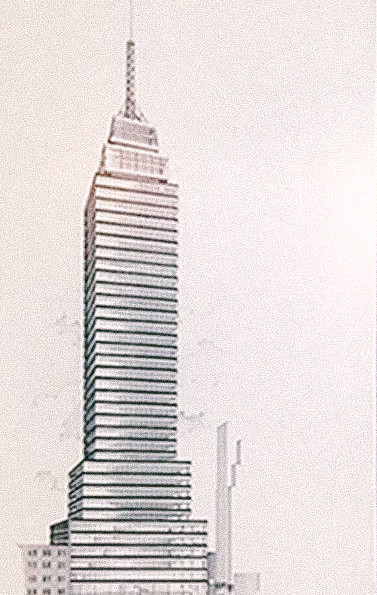
\includegraphics[scale=1.2]{Imagenes/Torre_Latino.jpg}
\end{figure}
\begin{tikzpicture}[overlay]
    \draw (7, 1.3) -- (7, 7) node [left, pos=1] {\small{$y$}};
    \draw (6, 1.3) -- (8, 1.3);
    \draw (6.7, 5.8) -- (7.3, 5.8);
    \draw [fill] (6.4, 5.8) circle (2pt);
\end{tikzpicture}
\end{frame}
\begin{frame}[plain]
\begin{figure}
\centering
\begin{tikzpicture}
    \draw (7, -1) -- (7, 7) node [left, pos=1] {\small{$y$}};

    \node at (2, 4) {\small{$a = -g = \SI{9.81}{\meter\per\square\second}$}};
    \draw [-stealth, thick] (2.5, 3.5) -- (2.5, 2.5);

    \draw (6, -1) -- (8, -1);
    \draw (6.7, 5.8) -- (7.3, 5.8);
    \draw [fill] (6.4, 5.8) circle (2pt);
    
    \node at (5.4, 5.6) {\small{$v_{0} = 0$}};
    \node at (8.5, 5.6) {\small{$t_{0} = 0 \quad y_{0}=0$}};
    \pause

    \draw (6.7, 4.8) -- (7.3, 4.8);
    \draw [fill] (6.4, 4.8) circle (2pt);
    \node at (5.4, 4.6) {\small{$v_{1} =$ ?}};
    \draw [-stealth, thick] (6.4, 4.8) -- (6.4, 4.3);
    \node at (8.5, 4.6) {\small{$t_{1} = \SI{1}{\second} \quad y_{1}=$?}};
    \pause

    \draw (6.7, 3) -- (7.3, 3);
    \draw [fill] (6.4, 3) circle (2pt);
    \draw [-stealth, thick] (6.4, 3) -- (6.4, 2.3);
    \node at (5.4, 2.8) {\small{$v_{2} =$ ?}};
    \node at (8.5, 2.8) {\small{$t_{2} = \SI{2}{\second} \quad y_{2}=$?}};

    \pause

    \draw (6.7, 1) -- (7.3, 1);
    \draw [fill] (6.4, 1) circle (2pt);
    \draw [-stealth, thick] (6.4, 1) -- (6.4, -0.5);
    \node at (5.4, 0.8) {\small{$v_{3} =$ ?}};
    \node at (8.5, 0.8) {\small{$t_{3} = \SI{3}{\second} \quad y_{3}=$?}};

\end{tikzpicture}        
\end{figure}
\end{frame}
\begin{frame}
\frametitle{Preparando la solución}
Tomaremos el origen $O$ como el punto de partida y la dirección hacia arriba como positiva.
\\
\bigskip
\pause
La coordenada inicial $y_{0}$ y la velocidad inicial $v_{0}$ son ambas cero.
\end{frame}
\begin{frame}
\frametitle{Preparando la solución}
La aceleración es hacia abajo, en la dirección $y$ negativa, \pause así que:
\pause
\begin{align*}
a = - g = - \SI{9.81}{\meter\per\square\second}
\end{align*}
Recordemos que por definición $g$ siempre es positiva.
\end{frame}
\begin{frame}
\frametitle{Preparando la solución}
Por lo que nuestras incógnitas son los valores de $y$ y $v$ en los tres instantes que indica el enunciado.
\end{frame}
\begin{frame}
\frametitle{La expresión a utilizar}
Tenemos las siguientes expresiones:
\pause
\begin{eqnarray*}
\begin{aligned}
y &= y_{0} + v_{0} \, t + \dfrac{1}{2} \, a \, t^{2} \\[0.5em] \pause
v &= v_{0} + a \, t 
\end{aligned}
\end{eqnarray*}
\end{frame}
\begin{frame}
\frametitle{La expresión a utilizar}
En un instante $t$ después de que se suelta la moneda, su posición y velocidad son:
\pause
\begin{eqnarray*}
\begin{aligned}
y &= 0 + 0 + \dfrac{1}{2} (-g) \, t^{2} = \pause (\SI{-4.9}{\meter\per\square\second}) \, t^{2} \\[0.5em] \pause
v &= 0 + (-g) \, t = \pause (\SI{-9.8}{\meter\per\square\second}) \, t
\end{aligned}
\end{eqnarray*}
\end{frame}
\begin{frame}
\frametitle{Ocupando los tiempos}
Cuando $t = \SI{1}{\second}$, se tiene que:
\pause
\begin{eqnarray*}
\begin{aligned}
y &= (\SI{-4.9}{\meter\per\square\second}) \, (\SI{1}{\second})^{2} = \pause \SI{-4.9}{\meter} \\[0.5em] \pause
v &= (\SI{-9.8}{\meter\per\square\second}) (\SI{1}{\second}) = \pause \SI{-9.8}{\meter\per\second}
\end{aligned}
\end{eqnarray*}
\end{frame}
\begin{frame}
\frametitle{Los resultados}
Luego de \SI{1}{\second}, la moneda está \SI{4.9}{\meter} debajo del origen ($y$ es negativa), \pause y tiene una velocidad hacia abajo ($v$ es negativa) con magnitud de \SI{9.8}{\meter\per\second}.
\end{frame}
\begin{frame}
\frametitle{Evaluación continua}
La posición y velocidad a los \SI{2.0}{\second} y \SI{3.0}{\second} se obtienen de la misma manera.
\pause
Demuestra que:
\begin{table}
\centering
\begin{tabular}{c | c | c}
Tiempo & Posición $(y)$& Velocidad $(v)$ \\ \hline
\SI{2.0}{\second} & \SI{-19.6}{\meter} & \SI{-19.6}{\meter\per\second} \\ \hline
\SI{3.0}{\second} & \SI{-44.1}{\meter} & \SI{-29.4}{\meter\per\second} \\ \hline
\end{tabular}
\end{table}
\end{frame}

\end{document}